\chapter{Návrh}
V této kapitole bude popsán návrh backendu, který se skládá s současného návrhu, navržených změn a návrhu chybějící funkcionality.
\section{Navržené úpravy}\label{navrh:upravy}
    V teto sekce budou navrženy změny návrhu vzhledem k nedostatkům aktuálního návrhu, které byly nalezeny během vývoje backendové a forntendové částí aplikace. 
    \subsection{Interval}\label{narh:upravy:interval}
    První změnou je nový návrh entity Interval. Původní návrh (viz. obrázek \ref{image:Interval1}) nevyhovoval svojí složitostí a zároveň jenom částečným pokrytím možných případů. Podrobněji teto problém je popsán v sekci \ref{analyza:pozadavky-frontendu}. Entita interval byla rozdělena do dvou entit. První entita (viz. obrázek \ref{image:Interval2}) úplně nahrazuje původní entitu. Druhou entitou je \textit{CareDayInterval} (viz. obrázek \ref{image:careDayInterval}), která reprezentuje časové rozmezí pečovatelských dnů.
    \begin{figure}\centering
	    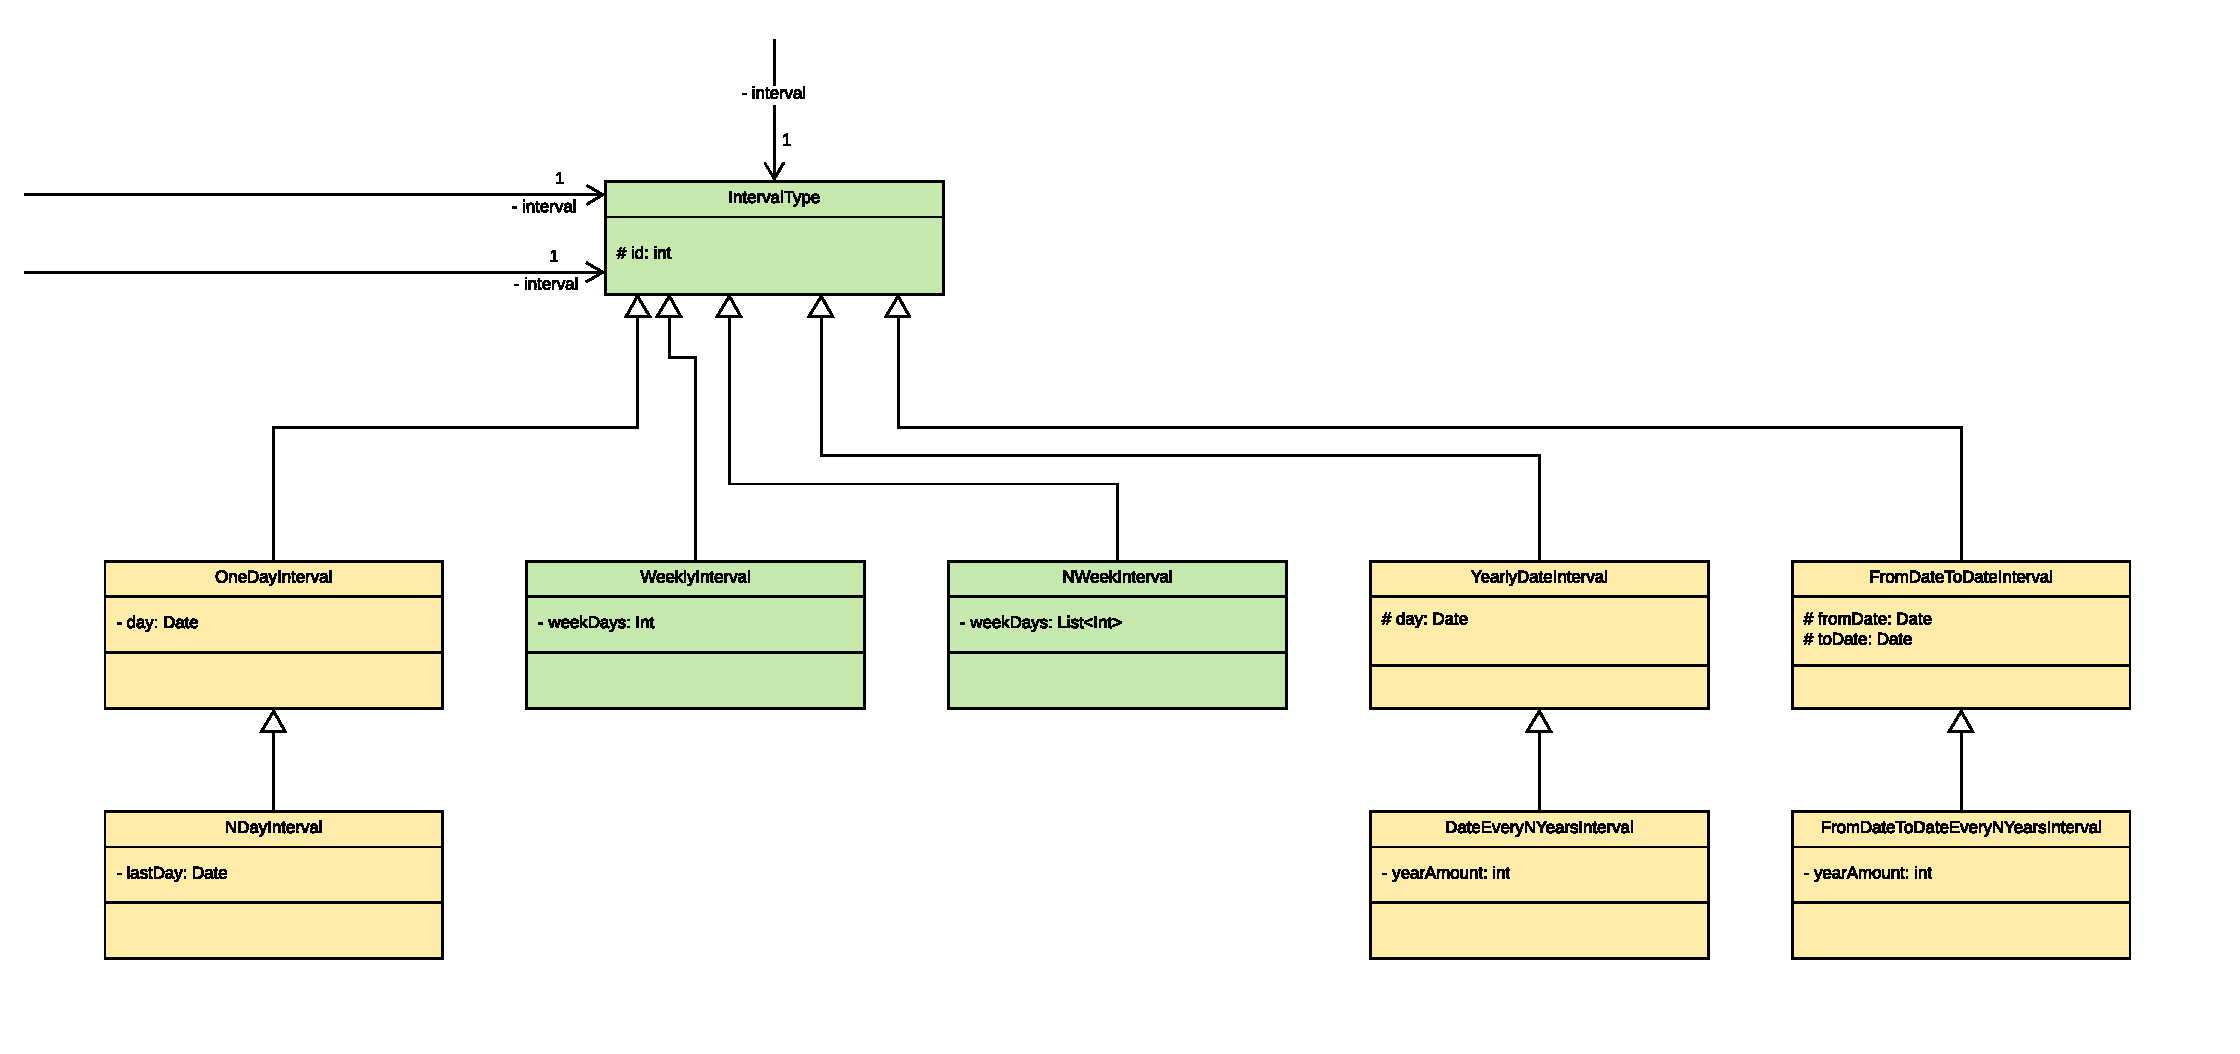
\includegraphics[width=1.0\textwidth]{pdfs/Interval1}
	    \caption[Návrh intervalu]{Návrh entity \textit{Interval} v Doménovém modelu z předmětu BI-SP2}\label{image:Interval1}
    \end{figure}
    \begin{figure}\centering
	    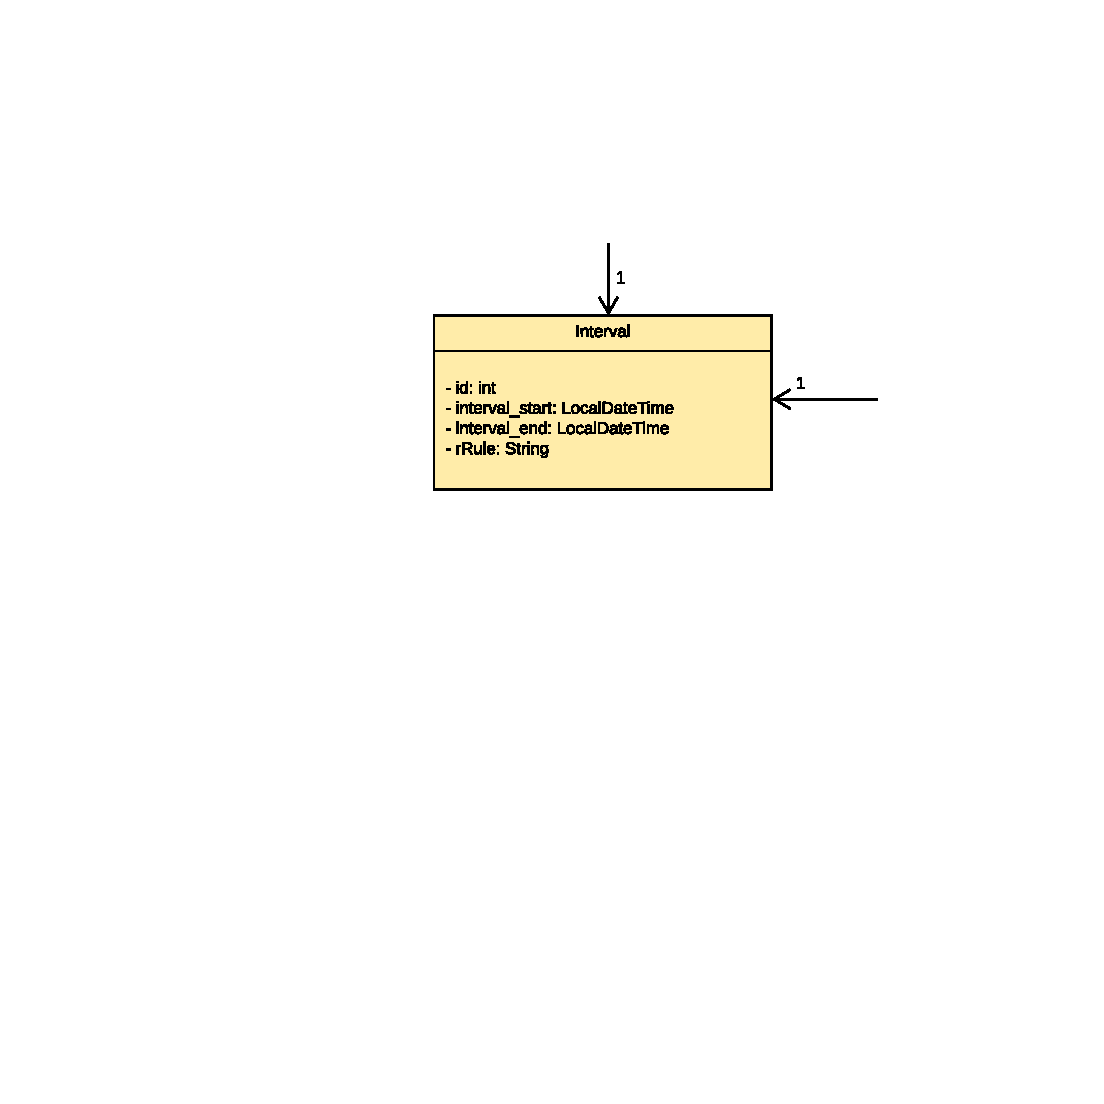
\includegraphics[width=0.5\textwidth]{pdfs/Interval2}
	    \caption[Návrh intervalu]{Nový návrh entity \textit{Interval}}\label{image:Interval2}
    \end{figure}
    \begin{figure}\centering
	    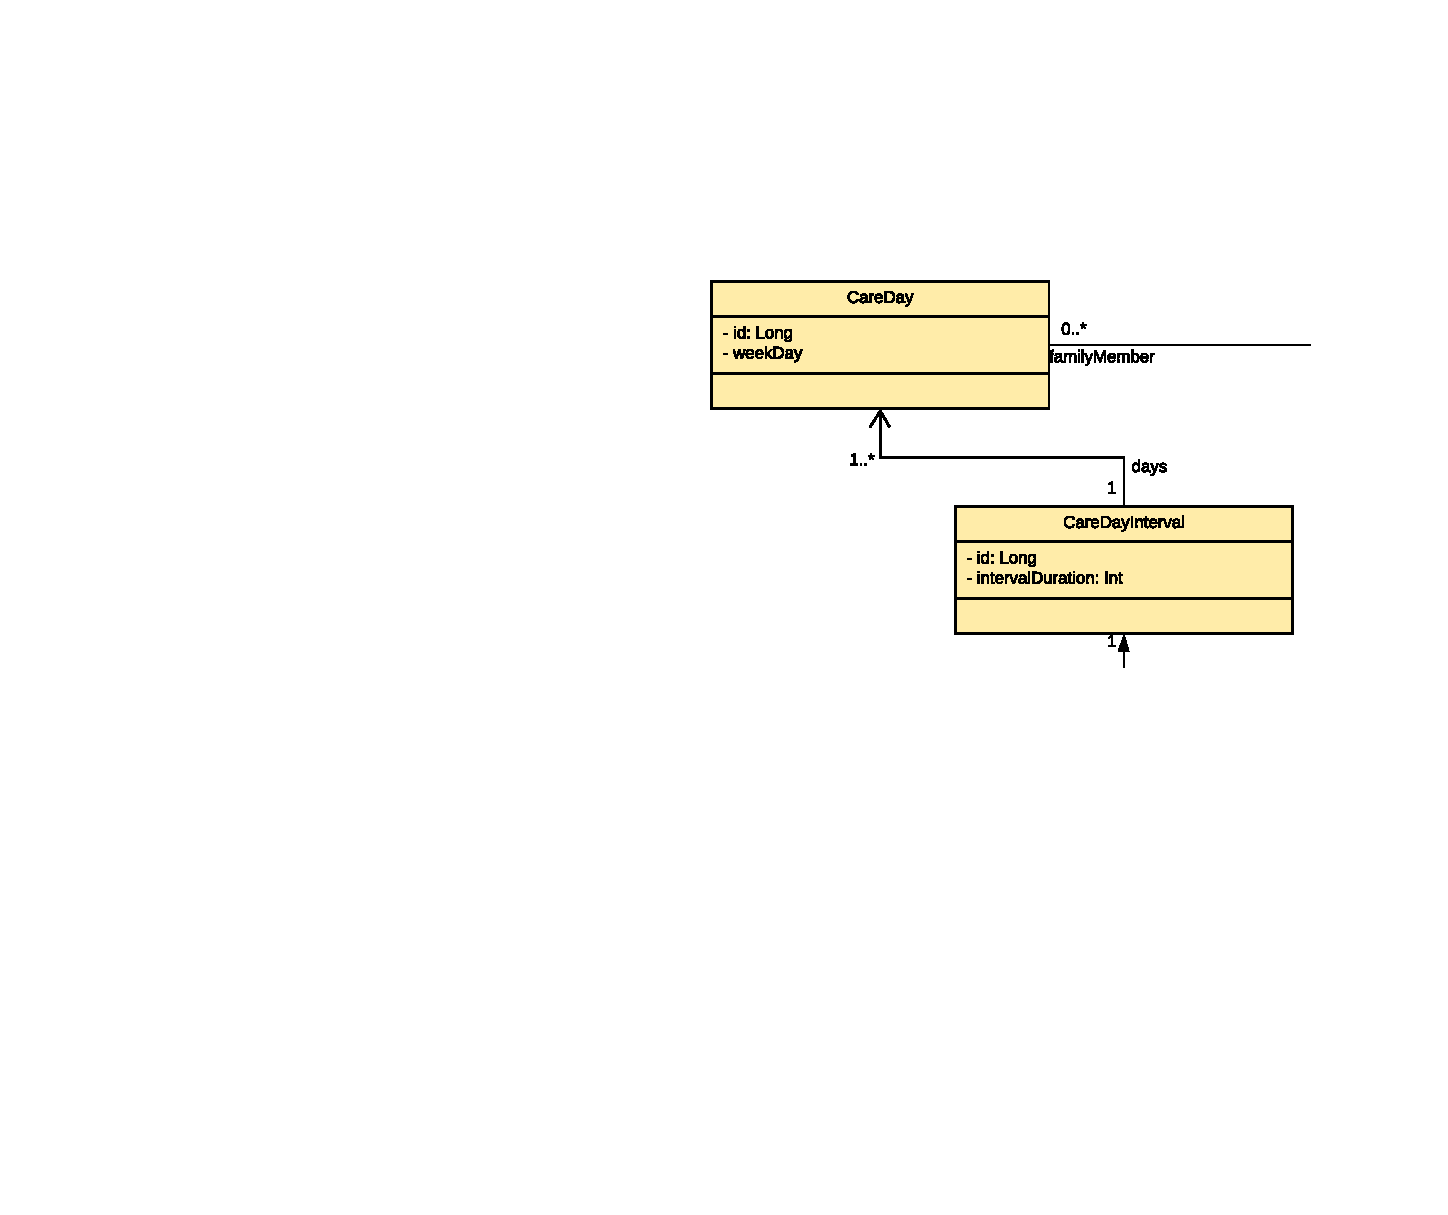
\includegraphics[width=0.5\textwidth]{pdfs/CareDayInterval}
	    \caption[Návrh intervalu]{Návrh entity \textit{CareDayInterval}}\label{image:careDayInterval}
    \end{figure}
    
    Nový návrh je postaven na úplně jiném principu. Časové rozmezí může být reprezentované dvěma způsoby. Oba dva způsoby vyžadují uvedení začátku intervalu. Tento parametr je povinný. První způsob, kromě začátku intervalu, vyžaduje i konec intervalu. Takovým způsobem můžeme definovat jednorázový interval po sobě jdoucích dnů. Druhý způsob vyžaduje zadání pravidlo opakování. Takhle můžeme definovat stejnou interval, ale mnohem složitějším způsobem. Na druhou stranu, pomocí takového pravidla můžeme definovat libovolně složitý interval. Takový návrh vyžaduje aby, buď byl zadán jenom konec intervalu, nebo bylo jenem zadáno pravidlo opakování. Pokud tyto dva parametry budou zadány najednou, server vyhodí chybu a zastaví vytvoření nesprávného intervalu.
    
    Pravidlo opakování je reprezentováno pomocí textového řetězce a má být zadáno ve standardu {RFC 5545}\cite{recurrence-rule}. Pro pohodlné testování byl navržen a implementován {interní DSL jazyk}\footnote{programovací jazyk nebo použití obecného programovacího jazyku, vytvořený za účelem vyřešení konkretní problémové domény}, který nadává možnost vytvořit pravidlo opakovaní. Dále uvádím příklad \textit{Intervalu}, který má pravidlo opakování vytvořené pomoci DSL jazyku. Tento interval bude použit při testování.
    \begin{figure}
        \begin{minted}{java}
        /**
        * Valid Interval with recurrence rule.
        */
        private val validInterval = Interval(
                id = 1,
                interval_start = creationTime,
                interval_end = null,
                rRule = rule(frequency = Frequency.WEEKLY, count = 10) {
                    byDays {
                        and(DayOfWeek.MONDAY)
                        and(DayOfWeek.WEDNESDAY)
                        and(DayOfWeek.SUNDAY)
                    }
                }
        )
        \end{minted}
        \caption{Ukázka \textit{Intervalu} s pravidlem opakování} 
        \label{code:valid-interval}
        \end{figure}
        %TODO popsat implemenaci interniho DSL
\section{Navrh bezpečnosti}\label{navrh:bezpecnost}

\section{Návrh testování}\label{navrh:testovani}
    Pro testování kódu budou využity frameworky JUnit 5 a Spring. Podrobný popis těchto frameworků byl v sekci \ref{resere:testovani}. Testování se skládá s \textit{Unit}\footnote{testy, zaměřené na ověření správnosti } testů a \textit{Integration}\footnote{TODO} testů.